\documentclass[14pt]{extbook}
\usepackage{multicol, enumerate, enumitem, hyperref, color, soul, setspace, parskip, fancyhdr} %General Packages
\usepackage{amssymb, amsthm, amsmath, bbm, latexsym, units, mathtools} %Math Packages
\everymath{\displaystyle} %All math in Display Style
% Packages with additional options
\usepackage[headsep=0.5cm,headheight=12pt, left=1 in,right= 1 in,top= 1 in,bottom= 1 in]{geometry}
\usepackage[usenames,dvipsnames]{xcolor}
\usepackage{dashrule}  % Package to use the command below to create lines between items
\newcommand{\litem}[1]{\item#1\hspace*{-1cm}\rule{\textwidth}{0.4pt}}
\pagestyle{fancy}
\lhead{Progress Quiz 4}
\chead{}
\rhead{Version B}
\lfoot{8448-1521}
\cfoot{}
\rfoot{Fall 2020}
\begin{document}

\begin{enumerate}
\litem{
Choose the equation of the function graphed below.
\begin{center}
    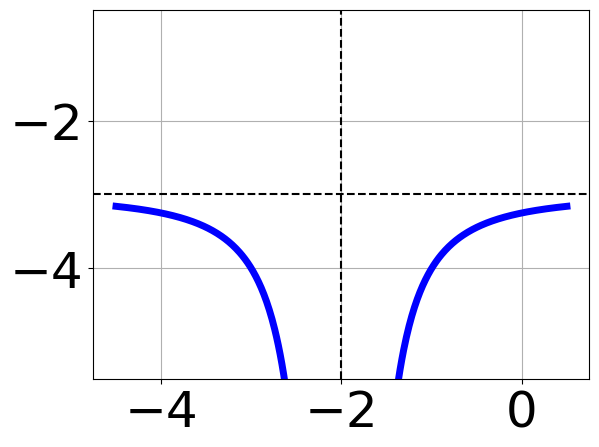
\includegraphics[width=0.5\textwidth]{../Figures/rationalGraphToEquationCopyB.png}
\end{center}
\begin{enumerate}[label=\Alph*.]
\item \( f(x) = \frac{-1}{(x - 3)^2} - 6 \)
\item \( f(x) = \frac{1}{(x + 3)^2} - 6 \)
\item \( f(x) = \frac{-1}{x - 3} - 6 \)
\item \( f(x) = \frac{1}{x + 3} - 6 \)
\item \( \text{None of the above} \)

\end{enumerate} }
\litem{
Determine the domain of the function below.\[ f(x) = \frac{6}{15x^{2} -15} \]\begin{enumerate}[label=\Alph*.]
\item \( \text{All Real numbers except } x = a \text{ and } x = b, \text{ where } a \in [-3, 0] \text{ and } b \in [1, 5] \)
\item \( \text{All Real numbers.} \)
\item \( \text{All Real numbers except } x = a, \text{ where } a \in [-28, -20] \)
\item \( \text{All Real numbers except } x = a, \text{ where } a \in [-3, 0] \)
\item \( \text{All Real numbers except } x = a \text{ and } x = b, \text{ where } a \in [-28, -20] \text{ and } b \in [9, 10] \)

\end{enumerate} }
\litem{
Solve the rational equation below. Then, choose the interval(s) that the solution(s) belongs to.\[ \frac{-6}{-5x -9} + -8 = \frac{-9}{15x + 27} \]\begin{enumerate}[label=\Alph*.]
\item \( x_1 \in [-1.88, -1.6] \text{ and } x_2 \in [-2.58,-0.57] \)
\item \( x \in [1.6,2.33] \)
\item \( x \in [-1.57,0.43] \)
\item \( \text{All solutions lead to invalid or complex values in the equation.} \)
\item \( x_1 \in [-1.59, -1.52] \text{ and } x_2 \in [1.02,3.02] \)

\end{enumerate} }
\litem{
Determine the domain of the function below.\[ f(x) = \frac{3}{18x^{2} +18 x -36} \]\begin{enumerate}[label=\Alph*.]
\item \( \text{All Real numbers except } x = a \text{ and } x = b, \text{ where } a \in [-18.1, -16.8] \text{ and } b \in [33.8, 37.6] \)
\item \( \text{All Real numbers except } x = a, \text{ where } a \in [-18.1, -16.8] \)
\item \( \text{All Real numbers.} \)
\item \( \text{All Real numbers except } x = a \text{ and } x = b, \text{ where } a \in [-3.3, -1.6] \text{ and } b \in [0.2, 1.8] \)
\item \( \text{All Real numbers except } x = a, \text{ where } a \in [-3.3, -1.6] \)

\end{enumerate} }
\litem{
Solve the rational equation below. Then, choose the interval(s) that the solution(s) belongs to.\[ \frac{20}{-45x + 15} + 1 = \frac{20}{-45x + 15} \]\begin{enumerate}[label=\Alph*.]
\item \( x \in [0.33,1.33] \)
\item \( \text{All solutions lead to invalid or complex values in the equation.} \)
\item \( x \in [-0.5,0.2] \)
\item \( x_1 \in [-0.2, 0.9] \text{ and } x_2 \in [-1.67,1.33] \)
\item \( x_1 \in [-0.5, 0.2] \text{ and } x_2 \in [-1.67,1.33] \)

\end{enumerate} }
\litem{
Solve the rational equation below. Then, choose the interval(s) that the solution(s) belongs to.\[ \frac{7x}{-2x -6} + \frac{-6x^{2}}{8x^{2} +32 x + 24} = \frac{7}{-4x -4} \]\begin{enumerate}[label=\Alph*.]
\item \( x_1 \in [0.45, 1.22] \text{ and } x_2 \in [-2.32,1] \)
\item \( x \in [-2.09,-1.04] \)
\item \( \text{All solutions lead to invalid or complex values in the equation.} \)
\item \( x_1 \in [0.45, 1.22] \text{ and } x_2 \in [-3.34,-2.32] \)
\item \( x \in [-1.21,-0.69] \)

\end{enumerate} }
\litem{
Solve the rational equation below. Then, choose the interval(s) that the solution(s) belongs to.\[ \frac{-6x}{-2x -4} + \frac{-5x^{2}}{6x^{2} -24} = \frac{-5}{-3x + 6} \]\begin{enumerate}[label=\Alph*.]
\item \( x_1 \in [-0.96, 0.54] \text{ and } x_2 \in [-3,2] \)
\item \( x_1 \in [-0.96, 0.54] \text{ and } x_2 \in [-0.07,4.93] \)
\item \( x \in [2.63,4.13] \)
\item \( \text{All solutions lead to invalid or complex values in the equation.} \)
\item \( x \in [1.45,2.86] \)

\end{enumerate} }
\litem{
Choose the graph of the equation below.\[ f(x) = \frac{-1}{(x - 1)^2} - 1 \]\begin{enumerate}[label=\Alph*.]
\begin{multicols}{2}\item 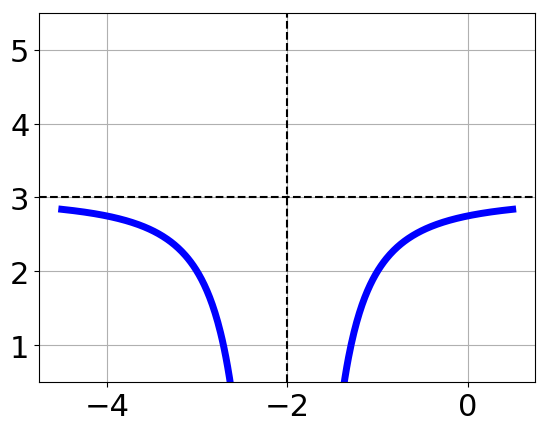
\includegraphics[width = 0.3\textwidth]{../Figures/rationalEquationToGraphAB.png}\item 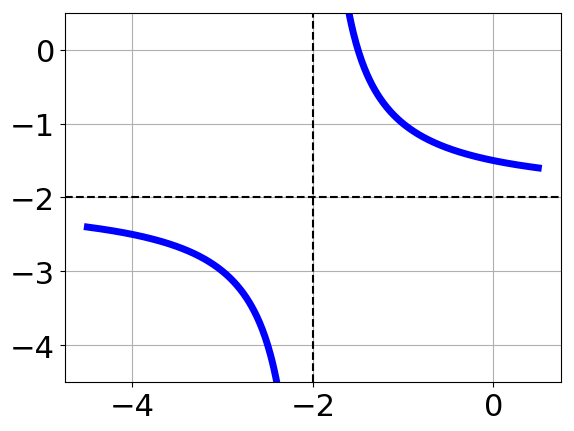
\includegraphics[width = 0.3\textwidth]{../Figures/rationalEquationToGraphBB.png}\item 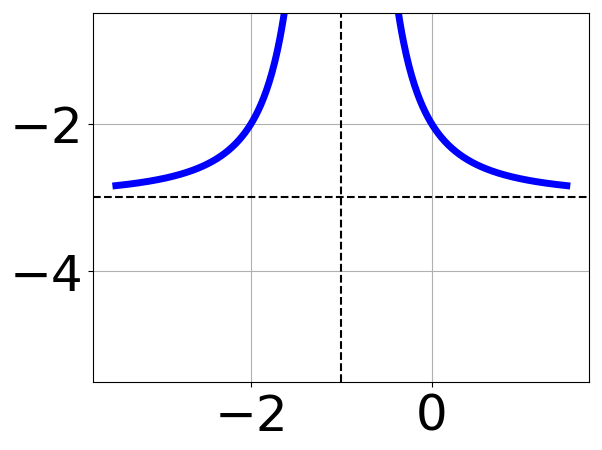
\includegraphics[width = 0.3\textwidth]{../Figures/rationalEquationToGraphCB.png}\item 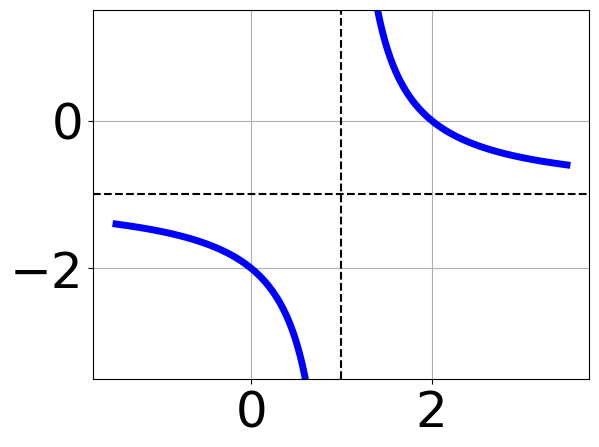
\includegraphics[width = 0.3\textwidth]{../Figures/rationalEquationToGraphDB.png}\end{multicols}\item None of the above.
\end{enumerate} }
\litem{
Choose the equation of the function graphed below.
\begin{center}
    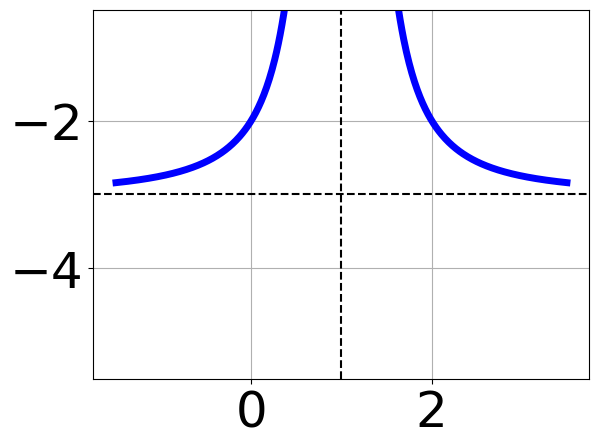
\includegraphics[width=0.5\textwidth]{../Figures/rationalGraphToEquationB.png}
\end{center}
\begin{enumerate}[label=\Alph*.]
\item \( f(x) = \frac{1}{(x + 2)^2} + 1 \)
\item \( f(x) = \frac{1}{x + 2} + 1 \)
\item \( f(x) = \frac{-1}{x - 2} + 1 \)
\item \( f(x) = \frac{-1}{(x - 2)^2} + 1 \)
\item \( \text{None of the above} \)

\end{enumerate} }
\litem{
Choose the graph of the equation below.\[ f(x) = \frac{-1}{(x + 2)^2} + 3 \]\begin{enumerate}[label=\Alph*.]
\begin{multicols}{2}\item 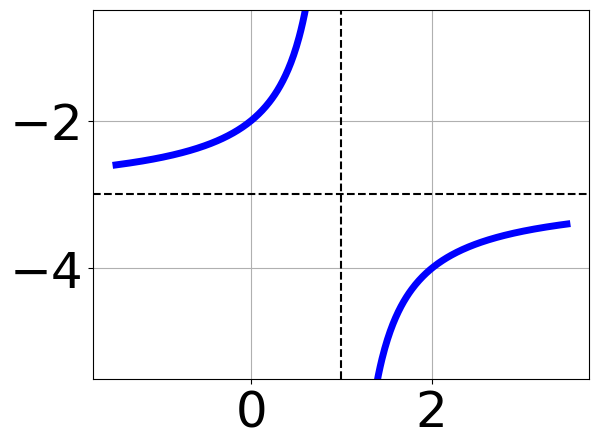
\includegraphics[width = 0.3\textwidth]{../Figures/rationalEquationToGraphCopyAB.png}\item 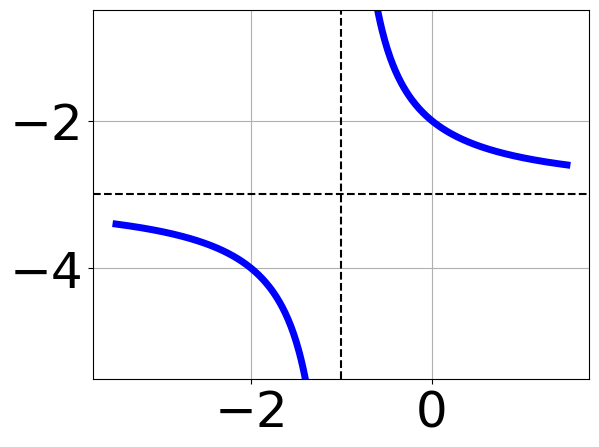
\includegraphics[width = 0.3\textwidth]{../Figures/rationalEquationToGraphCopyBB.png}\item 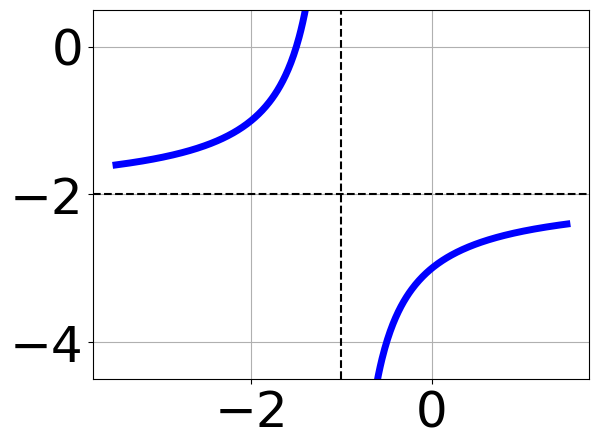
\includegraphics[width = 0.3\textwidth]{../Figures/rationalEquationToGraphCopyCB.png}\item 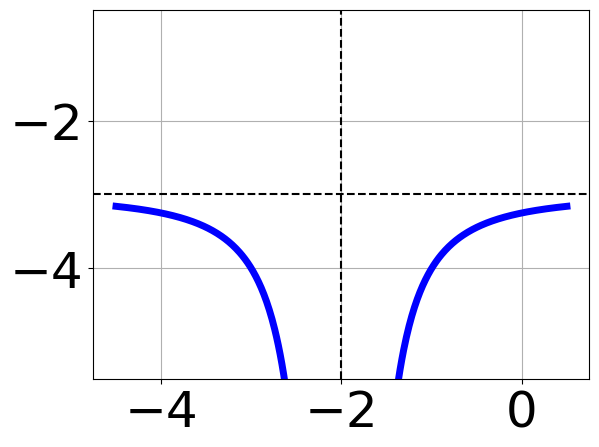
\includegraphics[width = 0.3\textwidth]{../Figures/rationalEquationToGraphCopyDB.png}\end{multicols}\item None of the above.
\end{enumerate} }
\end{enumerate}

\end{document}